\documentclass[a4paper, 11pt, compsoc]{IEEEtran}

\usepackage{amsmath}
\usepackage{physics}
\usepackage{hyperref}
\usepackage{cleveref}
\hypersetup{
	colorlinks = true,
	linkcolor = blue,
	filecolor = blue,
	citecolor = black,
	urlcolor = cyan,
}
\crefname{appsec}{Appendix}{Appendices}

\usepackage{graphicx}
\usepackage[section]{placeins}
\usepackage{bookmark}
\usepackage{gensymb}


%for code(MATLAB in particular)
\usepackage{listings}
\usepackage{color} %red, green, blue, yellow, cyan, magenta, black, white
\definecolor{mygreen}{RGB}{28,172,0} % color values Red, Green, Blue
\definecolor{mylilas}{RGB}{170,55,241}

\lstset{
    language=Matlab,%
    %basicstyle=\color{red},
    breaklines=true,%
    morekeywords={matlab2tikz},
    keywordstyle=\color{blue},%
    morekeywords=[2]{1}, 
    keywordstyle=[2]{\color{black}},
    identifierstyle=\color{black},%
    stringstyle=\color{mylilas},
    commentstyle=\color{mygreen},%
    showstringspaces=false,%without this there will be a symbol in the places where there is a space
    numbers=left,%
    numberstyle={\tiny \color{black}},% size of the numbers
    numbersep=7pt, % this defines how far the numbers are from the text
    emph=[1]{for,end,break},
    emphstyle=[1]\color{red}, %some words to emphasise
    %emph=[2]{word1,word2}, emphstyle=[2]{style},
}


\graphicspath{{./pictures/}}

\title{ECEN315 - Open Loop Response of a Motorised, Propeller Driven Pendulum}
\author{Joshua Benfell - 300433229}

\IEEEtitleabstractindextext{
    \begin{abstract}
        This report covers the derivation of the open loop response for a properller driven pendulum for the purpose of understanding how such a system will respond to an applied voltage at the motor. The methods for doing such a derivation are provided as well as the simulated response of the system to various step inputs. Beyond that areas where error was introduced into the model are discussed along with the effect of changing those values. Evaulation is then done on whether the model is a suitable representation of the physical equivalent. Finally expectations of a physical system are presented along with the possibility of designing a PID controller in a future study and where a similar system might be applied.
    \end{abstract}
}


\begin{document}
    \maketitle
    \IEEEdisplaynontitleabstractindextext

    \section{Introduction}\label{sec:intro}
        The aim of this report is to derive the theoretical open loop response for a motorised, propeller driven pendulum arm. By deriving this, we aim to understand how such a pendulum responds to an applied voltage. From this an understanding of the real system will be gained along with the shortcomings of the model representing that system.
        \par
        \cref{sec:bg} will cover some control theory and terms to aid the understanding. \cref{sec:methods} is where the process to derive the transfer function of this system is coevered. \cref{sec:results} will present the results of the model and discuss them and the system. \cref{sec:conclusion} will present a summary of the results as well as the follow up to deriving this model.

    \section{Background}\label{sec:bg}
        \begin{figure}[!h]
            \centering
            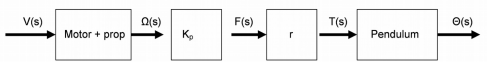
\includegraphics[width=\columnwidth]{overallBlockDiagram.png}
            \caption{Block diagram for full system}
            \label{fig:fullBlockDiagram}
        \end{figure}
        An open loop system is a system where the output is not fed back into the system. The alternative is a closed loop system where the input is fed back into the system, typically subtracted from the input to get the error. The full system (\cref{fig:fullBlockDiagram}) that this paper will be modelling can be done so as an open loop system. While the overarching system is an open loop system, some of the systems that make up the blocks are themselves, closed loop systems, while others are open loop systems.
        \par
        \begin{figure}[!h]
            \centering
            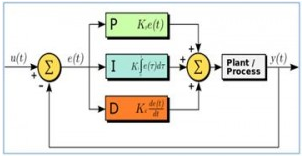
\includegraphics[width=\columnwidth]{PID.png}
            \caption{Diagram of a PID Controller \cite{elprocus}}
            \label{fig:pid}
        \end{figure}
        An example controller that could be implemented with this system to make it a closed loop system is a proportional, integral, derivative (PID) controller. This controller has three components to it all revolving around the error. In this closed loop system, the final output is subtracted from the input resulting in the error, as mentioned above. Putting this through a gain (P) controller, which is just represented as a constant value, will help make the system more responsive, however, there is a consequence of making the system more oscillatory and leaving the system with a steady state error (the difference between target and output). The I controller integrates over all errors (also multiplies by a gain constant) and aims to remove the steady state error, it also can speed up the response. This is done by lowering the gain of the controller. The D controller, differentiates over the error and allows the controller to predict the future of the system, and react earlier making it more responsive. Summing these all together provides a PID signal which is then put into the plant instead of the original input \cite{elprocus}. Something like this is the eventual goal with the modelled system.
        \par
        One of the evaluated characteristics of this system is it's stability. Stability of a system is defined as whether or not the output grows without bounds, if it does then the system is unstable, whereas it is stable if it settles on a value. This is regardless of any oscillation that would occur in the system. Stability can also be pre-determined by looking at the poles of the system, i.e. the values of $s$ that make the denominator of the transfer function $0$. If the real component of the poles is negative then the system is stable and vise versa if it is positive.        
        % \par
        % Design, solving, and evaluation of systems is typically done in the frequency domain.  


    \section{Method}\label{sec:methods}
        \begin{figure}[!h]
            \centering
            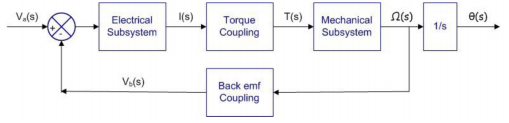
\includegraphics[width=\columnwidth]{motorTF.png}
            \caption{Block diagram that describes the motor response to an applied voltage. \cite{gouws_2008}}
            \label{fig:motorBlockDiagram}
        \end{figure}
        
        The block diagram in \cref{fig:fullBlockDiagram} illustrates an approximation of the full powered pendulum system. This system takes an input voltage into the motor causing the shaft to spin with angular velocity $\omega(t)$. Due to the propeller on the motor, this speed at which the shaft spins will generate a force which is represented by the constant $K_p$. The torque is then obtained by mutliplying by the distance from the pivot to the center of the motor. Finally this torque is applied to the pendulum arm, resulting in an angular displacement of the arm.
        \par

        \begin{figure}[]
            \centering
            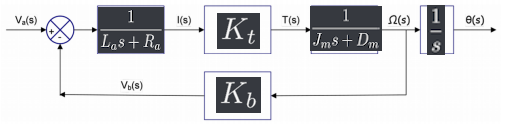
\includegraphics[width=\columnwidth]{full.png}
            \caption{Block diagram for motor and prop with equations in corresponding blocks \cite{gouws_2008}}
            \label{fig:motorBlockDiagramValues}
        \end{figure}
        The first block to look at is the one that describes how the motor responds to an applied voltage. This behaviour can be broken down into smaller sub-systems as shown in \cref{fig:motorBlockDiagram}.Each of those systems can be filled with the appropriate transfer function consisting of measurable properties of the motor with propeller as show in \cref{fig:motorBlockDiagramValues} where:
        \begin{itemize}
            \item $L_a$ is the inductance of the armature
            \item $R_a$ is the resistance of the armature
            \item $K_t$ is the torque constant that relates the current to the torque produced
            \item $J_m$ is the inertia of the load (propeller)
            \item $D_m$ is the damping coefficient of the load (propeller)
            \item $K_b$ is the back emf constant, relating the angular velocity to an induced voltage.
        \end{itemize}
        
        The block diagram can be simplified into a generic transfer function (\cref{eq:motorTF}) the represents the response of the motor to an applied voltage (See \cref{app:motorDerivation} for full derivation). This transfer function was then plugged into MATLAB and evaluated with step inputs of amplitude 2, 3, 4, 5 and 6V.
        \begin{equation} \label{eq:motorTF}
            \frac{\Omega(s)}{V(s)} = \frac{\frac{K_t}{J_mL_a}}{s^2  + \frac{J_mR_a + D_mL_a}{J_mL_a}s + \frac{R_aD_m+K_tK_b}{J_mL_a}}
        \end{equation}

        \begin{figure}[!h]
            \centering
            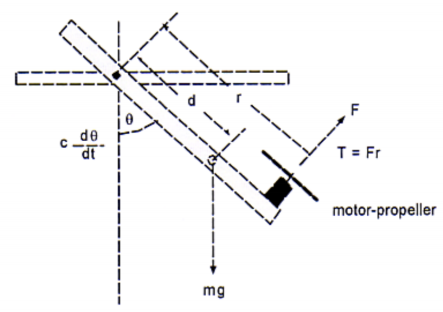
\includegraphics[width=\columnwidth]{pendulum.png}
            \caption{Diagram of the powered pendulum}
            \label{fig:pendulum}
        \end{figure}

        The next block to expand upon is the one that represents the pendulums response, as the two in the middle are just constants. For this block, a force is being applied (from the motor) which results in the angular displacement of the pendulum arm. An expression for net torque ($\tau_{net} = \alpha J_p$) must then be derived. Using the diagram in \cref{fig:pendulum}, it can be seen that there are three main torques acting on the arm; The torque from the propellered motor ($\tau_m = Fr$), the torque induced by friction around the pivot when the arm is moving ($\tau_f = c\dv{\theta}{t}$) and the component of the gravity vector that is perpendicular to the arm ($\tau_g = dmg\sin{\theta}$). 
        \par
        Combining the different torques of the system into one equation allows us to find an expression for the torque produced by the motor (\cref{eq:secondOrderDE}). After making the assumption that $\sin{\theta} = \theta$ and that $\alpha$ is the second derivative of angular displacement, \cref{eq:secondOrderDE} takes the form of a second order homogeneous ordinary differential equation. Applying the Laplace transform to this equation allows us to rearrange it so that it resembles a transfer function with angular displacement as the output to an applied torque (\cref{eq:pendulumTF}).

        \begin{equation}\label{eq:secondOrderDE}
            \begin{split}    
                \tau_{net} = & \tau_m - \tau_f - \tau_g \\
                \tau_m = & \tau_{net} + \tau_f + \tau_g \\ 
                \tau_m = & \alpha J_p + c\dv{\theta}{t} + dmg\sin{\theta} \\ 
                \tau_m =  & J_p \dv[2]{\theta}{t} + c\dv{\theta}{t} + dmg\sin{\theta} \\
                \tau_m =  & J_p \dv[2]{\theta}{t} + c\dv{\theta}{t} + dmg\theta
            \end{split}
        \end{equation}

        \begin{equation}\label{eq:pendulumTF}
            \frac{\Theta(s)}{\rm T(s)} = \frac{\frac{1}{J_p}}{s^2 + \frac{c}{J_p}s + \frac{dmg}{J_p}}
        \end{equation}

        \begin{figure}
            \centering
            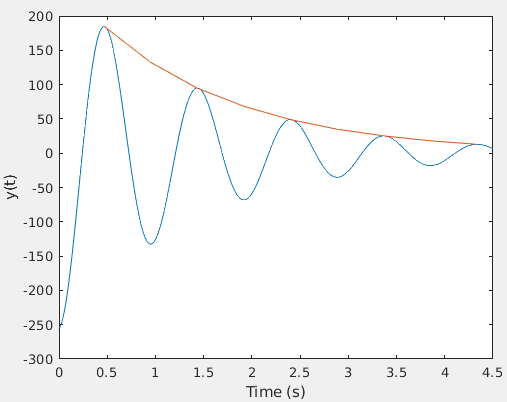
\includegraphics[width=\columnwidth]{plottedPendulumData.png}
            \caption{Undriven penudulum data with peaks connected to resemble an exponential}
            \label{fig:pendulumData}
        \end{figure}

        Before plotting this in MATLAB for evaluation, the value for each variable need to be found. For $d$, $m$ and $g$ this is relatively easy as it is just measuring the distance to the center of mass, weighing it and using the constant value for gravity on earth of $9.81 \frac{m}{s^2}$. To find $J_p$ and $c$ the pendulum was let to fall and the oscillation recorded. An exponential was then fit through the peaks of the plot (\cref{fig:pendulumData}) to find the values of $A$ and $B$ in \cref{eq:dampedPendulumEq} using the non-linear model (nlm) function in MATLAB (Can also see \cref{app:AB} for a manual method). \cref{eq:dampedPendulumEq} is the equation that models the motion of the pendulum where $\omega$ is given by \cref{eq:omega}. When finding $A$ and $B$, only the non-oscillitary component of \cref{eq:dampedPendulumEq} is important and used. Once found, \cref{eq:omega} can be rearranged for $J_P$ and then $c = 2BJ_p$.
        
        \begin{equation}\label{eq:dampedPendulumEq}
            \begin{split}
                y & = A e^{-\frac{c}{2J_p}t} \cos(\omega t + \phi) \\
                  & = A e^{-Bt}\cos(\omega t + \phi) 
            \end{split}
        \end{equation}

        \begin{equation}\label{eq:omega}
            \begin{split}
                \omega & = \sqrt{\frac{mgd}{J_p} - \left(\frac{c}{2J_p}\right)^2} \\ 
                  & = \sqrt{\frac{mgd}{J_p} - B^2}
            \end{split}
        \end{equation}

    \section{Results and Discussion}\label{sec:results}
        \subsection{Motor Response}
            \begin{figure}[!h]
                \centering
                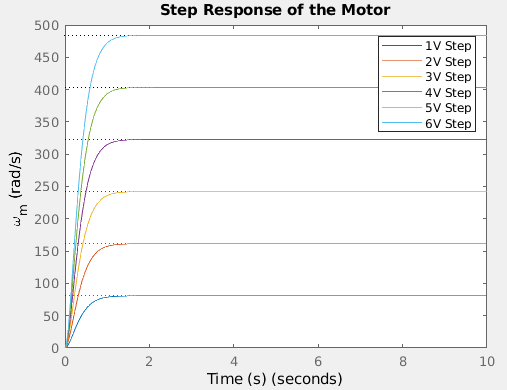
\includegraphics[width=\columnwidth]{motorStepResponse.png}
                \caption{Step response of the motors transfer function}
                \label{fig:motorStepResponse}
            \end{figure}
            \begin{figure}[!h]
                \centering
                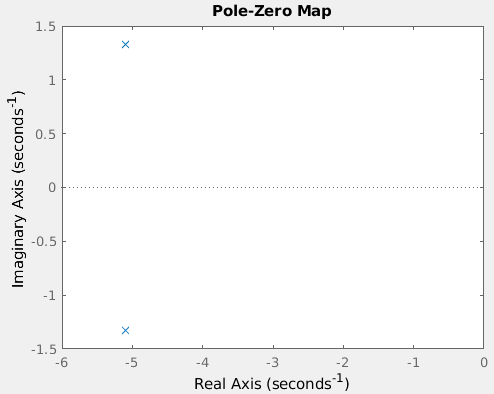
\includegraphics[width=\columnwidth]{motorPZMap.png}
                \caption{PZ Plot of the motors transfer function}
                \label{fig:motorPZ}
            \end{figure}
            \begin{table}
                \centering
                \caption{Table of Motor Parameters}
                \label{tab:motorValues}
                \begin{tabular}{l|r}
                    Motor Parameters  & Value\\
                    \hline
                    $R_a (\Omega)$ & $6.3$\\
                    $La (H)$ & $0.797$ \\
                    $Kb (V.s/rad) = Kt (N.m/A)$ & $0.0043$ \\
                    $Dm (N.m.s/rad)$ & $0.00000553$ \\
                    $Jm (kgm2)$ & $0.00000241$
                \end{tabular}
            \end{table}
            Step inputs ranging from 1V to 6V were applied to the transfer function of the motor (\cref{eq:motorTF}) using the provided values in \cref{tab:motorValues}, the resulting plot is \cref{fig:motorStepResponse}. From this plot it can be seen that the motor winds up to a final angular velocity. The steady state gain of the motor is $80.6316 [radians/Volt second]$ which means that each steady state value is the step inputs amplitude multiplied by the gain. The motor settles on this after $1.0374 s$ with a time constant of $0.196 s$ (found by $\frac{1}{\omega_n \zeta}$).
            \par
            Looking at \cref{fig:motorPZ} shows that the response of a motor with the parameters given in \cref{tab:motorValues} is complex and oscillitary. However, the step response indicates that this is a very small and insignificant oscillation that makes the system indistiguishable from one with purely real poles.
            \par
            As mentioned prior, the parameter values in \cref{tab:motorValues} were provided for this experiment. They are the result of averaging prior similar experiments measurements. With this comes room for error as each motor has it's own independent properties.
            \par
            Error around $R_a$ and $L_a$ exists because these are values that vary as the motor spins due to the connection between the coils and brushes changing as they become more and less connected. So if not enough measurements were taken with the motor shaft in different positions, the average of those points could be further off from the true value. If these values are to change then the damping and steady state gain of the system are subject to change. The steady state gain depends on $R_a$ of the two variables currently being discussed, an increase in this causes a decrease in the gain. It also causes and increase in damping. If $L_a$ were to increase then the damping from the resistive component of the motor will decrease.
            \par
            $K_b$ and $K_t$ can be measured by measuring the voltage across the motor and dividing by the angular velocity of the motor \cite{gouws_2008}. This introduces errors through the measuring apparatus. If a tachometer was used then the refresh rate of the device and how reflective the propeller and background are could effect the readings. If a spectrum analyser was used then microphone quality and distance are the main factors, but it is possible to get a more accurate reading. However, it's uncertain how these values were obtained. If the measured values $K_t$ or $K_b$ change, then the other will two as they are equivalent \cite{gouws_2008}, this changes affects the steady state gain and an increase will decrease the gain more than it increases it.
            \par
            Measuring $D_m$ encounters the same problems as $K_b$ and $K_t$ as shown in \cite{gouws_2008}. If this variable increases then the damping of the system also increases, as this is the damping coefficient, and the steady state gain decreases as this increase indicates a possible decrease in angular velocity.
            \par
            $J_m$ errors can arise from the measurement in $D_m$ and however the mechanical time constant is measured. If this value would increaes then the damping would decrease due to less being less susceptible to change.
            \par
            \begin{figure}[!h]
                \centering
                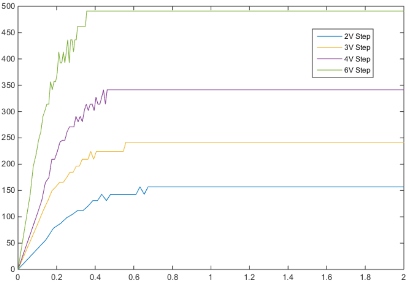
\includegraphics[width=\columnwidth]{exampleMotorResponse.png}
                \caption{Example Step response of the physical motor}
                \label{fig:exampleMotor}
            \end{figure}
            The motor response from this experiment \cref{fig:motorStepResponse} can be directly compared to the response from a prior experiment \cref{fig:exampleMotor}. From the previous response it is shown that this experiments theoretical response matches the response of a physical motor in overall shape. The pysical response has some mechanical distortions in it that are difficult to model. The settling time appears to shorten with higher steps in \cref{fig:exampleMotor} which is a limitation of the model provided by this report as \cref{fig:motorStepResponse} shows a constant settling time.
        \subsection{$K_p$}
            This coefficient affects the gain of the overall pendulum system and is linearly proportional to it. It's found by measuring the steady state force exerted by the propeller arm for a given input voltage and has units $\frac{Ns}{rad}$. Any error that could be introduced here comes from the accuracy of measurements.
        \subsection{r}
            This coefficient affects the gain of the overall pendulum system and is linearly proportional to it. It is found by using a ruler and any error is in the measurement and accuracy of the measurement.
        \subsection{Pendulum}
            \begin{figure}[]
                \centering
                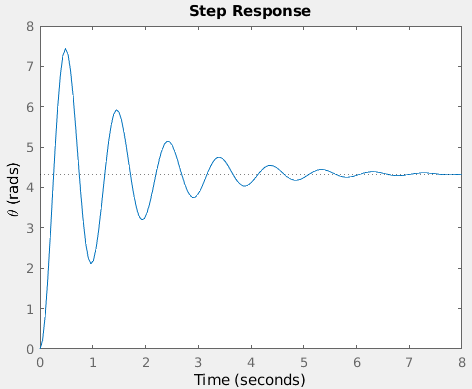
\includegraphics[width=\columnwidth]{pendulumStepResponse.png}
                \caption{Step response of the pendulum transfer function}
                \label{fig:pendulumResponse}
            \end{figure}
            Using the methods described in the pendulum section of \cref{sec:methods} (and \cref{app:AB}), c was found to be $0.0075 \frac{kg m^2 s}{rad}$ and $J_p$ was found to be $0.0054 \frac{rad}{kg m^2 s}$. The step response (for an applied torque of $1Nm$) to the system is \cref{fig:pendulumResponse} and indicates that adding this to the rest of the system will add a greater oscillatory component. This response is far too large for the model to realistically hold up, for the inputted torque as the pendulum does a full 360 before springing back past the origin. 
            \par
            The data used to model this was also supplied similar to the other aforementioned parameters. I am unable to comment on areas for error with this data as I am unsure on it's origin. It could be synthesised or measured and depending on which one indicates the level of error present. On top of that the data has been provided unitless so there is a lack of certainty on what the y axis is measuring, as the x axis can be assumed to be time. However, the effects of these variables changing can be discussed. Should $c$ increase the amplitude of oscillations in the pendulum will decrease as the system is more damped. Should $J_p$ increase, then the amplitude of the oscillations will increase as the system becomes less damped and more resistant to changes. 
            \par
            The other variables important to this transfer function are $d$ the distance from the pivot to the center of mass, $g$ the acceleration due to gravity which can be assumed to be the constant of $9.81 \frac{m}{s^2}$ and $m$ the mass of the arm. Error can come from the accuracy of these measurements, and g, realistically changes as the arms moves, but it is typically not enough to care about in this situation as the arm is short. However, these values are unlikely to vary greatly between similarly constructed arms, and will only do so otherwise.
        \subsection{Combined System}\label{sec:combined}
            \begin{figure}
                \centering
                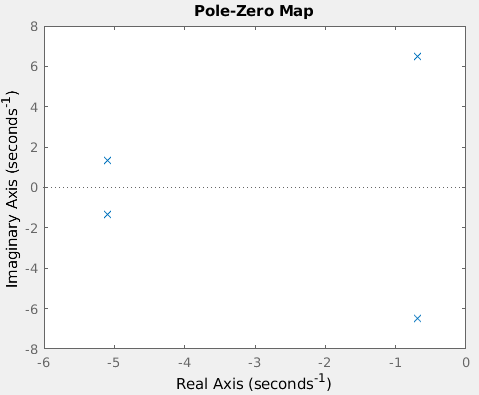
\includegraphics[width=\columnwidth]{fullSystemPZ.png}
                \caption{Poles and Zeroes of the Final System}
                \label{fig:fullPZ}
            \end{figure}
            \begin{figure}
                \centering
                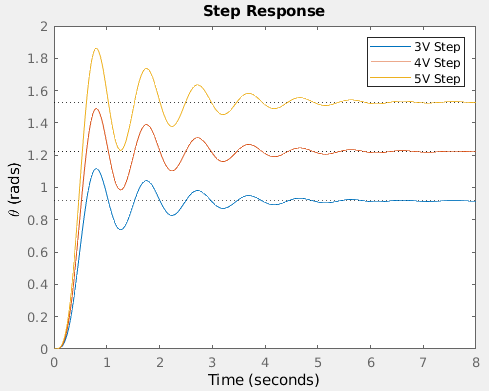
\includegraphics[width=\columnwidth]{fullSystemResponse.png}
                \caption{Step Response of the Final System}
                \label{fig:fullStepResponse}
            \end{figure}

            Combining all the major blocks in this system results in a transfer function that looks like \cref{eq:fullTF}. From this transfer function and the pole-zero plot (\cref{fig:fullPZ}), the system is expected to be stable and underdamped with, from the transfer function, a steady state gain of $\frac{K_tK_pr}{dmgR_aD_m + dmgK_tK_b} = 0.3056 rad/V$. This assumption aligns with the results of the two major non-coefficient systems as well, as these are both oscillatory and stable. Using the linear system analyser in MATLAB shows that the steady state gain is indeed this value and that each system has a settling time of $4.28s$. Additionally, from \cref{fig:fullStepResponse}, where the system was plotted for step inputs of size $3V$, $4V$ and $5V$, the system is is visibly underdamped and stable. Each of these steps has a final value of $52.53 \degree$, $70.04 \degree$ and $87.55 \degree$ respectively.
            \par
            A settling time of $4.28s$ indicates that this system is going to be oscillating quite violently as that's the time it takes 4 oscillations to happen, and as input voltage is increased, the amplitude of these oscillations also does. 

            \begin{equation}
                \label{eq:systemDenom}
                \begin{aligned}
                    V(s) = s^4 + \frac{ J_pJ_mR_a + J_pD_mL_a + J_mL_ac }{J_pJ_mL_a}s^3 + \\
                    \frac{R_aD_mJ_p + K_tK_bJ_p + J_mR_ac + D_mL_ac + dmgJ_mL_a}{J_pJ_mL_a}s^2 + \\
                    \frac{R_aD_mc + K_tK_bc + dmgJ_mR_a + dmgD_mL_a}{J_pJ_mL_a}s + \\
                    \frac{dmgR_aD_m + dmgK_tK_b}{J_pJ_mL_a}\\
                \end{aligned}
            \end{equation}

            \begin{equation}
                \label{eq:fullTF}
                \begin{aligned}
                    \frac{\Theta(s)}{V(s)} = \frac{ \frac{K_tK_pr}{J_pJ_mL_a} }{ \cref{eq:systemDenom} }
                \end{aligned}
            \end{equation}
        
        
        \subsection{Shortcomings of the model}
            As mentioned in \cref{sec:methods}, an assumption that needed to be made to simplify the differential equation was that $\sin{x} = x$. This assumption is typically done for very small angles as it encompasses the linear section of a sinusoid and is valid for up to $20\degree$ as beyond that the error gets too large \cite{russel_2020}. Because of this assumption, it is expected that a real system, the torque from gravity will have less of an impact causing the pendulum to have greater oscillations or oscillate for longer, and a higher steady state gain. This is particularly important as the settling angles of our model for the given step inputs are beyond the point where this assumption starts to break.
            \par 
            Another simplification made by this model is the drag on the propeller. In this model the drag is modelled as the linear relation $c\dv{\theta}{t}$, where $c$ is the proportionality constant that is assumed to represent friction and drag, if it just represents drag then that is another shortcoming of this model. For a real system, a more accurate model for the drag is that it is proportional to $V^2$ or $\dv{\theta}{t}^2$ \cite{Gupta2018}. This means that a real system is expected to take longer to settle the higher the applied voltage (from resting) as the higher voltage would incite a faster initial speed. From this increased drag, the size of the oscillation would be reduced as the system is now more damped and not going as fast to cause as big of an overshoot.
            \par
            From these two limitations of the model, it becomes inaccurate for the step values used in the plot \cref{fig:fullStepResponse}. This is because the system, responds with a higher angular displacement than the model allows for. So for small input voltages this model will hold up as the output angle will be closer to falling in an acceptible range for one of the assumptions. This also covers the other assumption around drag, as the pendulum arm won't be going fast enough to need to consider the $V^2$ component and leaving it as a linear relationship will be good enough.
            \par
            Due to the various amounts of error sources stated in the above sections, the model is unable to accurately represent a real system. This isn't so much of an issue as it still allows a general representation of how a system, that resembles the one described in this report, will respond as the values are taken from real systems and are within the correct range. This means that real systems will have different amounts of damping, response times, overshoots, periods etc.
        
    % \section{Discussion}\label{sec:discussion}
    \section{Conclusion}\label{sec:conclusion}
        In this report the process to derive and model a propellor driven pendulum was presented. This model was then used and evaluated, primarily the potential sources of error and how variations in measurements would affect the system, and the accuracy of the model. The resulting model was found to be oscillatory and stable and provided a good representation of the system, for small input voltages as this would produce a small output angle. Due to the large amount of room for error with the amount of variables that can change from system to system, it is expected that a physical system will have variation in it's response, but will maintain the same overall shape of response.
        \par
        Following on from this report, the next step is to model a potential control system for the system modelled in this report. The control systems aim will be to smoothly transistion the arm from one angle to another selected by the user. By making this model, the ground work will be laid out for other implementations of a PID controller for controlling angular position in pendulum type construction, such as an inverted pendulum or legs.


    \Urlmuskip=0mu plus 1mu\relax
    \bibliography{bibliography}
    \bibliographystyle{IEEEtran}

    \onecolumn
    \appendices
        \crefalias{section}{appsec}
        \section{Matlab Code}
            \lstinputlisting{../lab2.m}
            \lstinputlisting{../lab3.m}
        \section{Risk Assessment}

            \begin{table}
                \centering
                \begin{tabular}{p{4.5cm}|p{3cm}|l|l|p{4.5cm}}
                    \textbf{Hazard} & \textbf{Cause} & \textbf{Probability} & \textbf{Severity} & \textbf{Mitigation} \\
                    \hline
                    Getting fingers/jeans etc. cut by Spinning propellor & Turning the fan on & Unlikely & Low & Turn fan off when not in use. Don’t stick your finger in the path of the blade. \\
                    \hline
                    Hot motors & Running motors too long & Unlikely & Low & Don’t run the motor for too long and turn off when not in use \\
                    \hline
                    Tripping on cables & Walking over areas that have cables on the floor. E.g. getting fan box & Likely & Medium & Watch where you are walking if there are cables on the ground. \\
                    \hline
                    Electric shocks/shorts & Power supplies, exposed wires. & Likely & Medium & Be aware of exposed wires that have a potential over them. Don’t turn the power supplies too high. Don’t touch exposed cables if you can conduct. Don’t stick a fork in mains. \\
                    \hline
                    Integral wind up & Leaving fan off for a while with program running, then turning on. & Likely & High & Reset the program if the fan has been off for a while. Include some limitations/safety in code. \\
                    \hline
                    Lego pains. Things stuck in feet & Not wearing shoes & Unlikely & Low & Wear shoes \\
                    \hline
                    general toxic fumes & Soldering & Likely & High & Well ventilated and don’t breath in the fumes \\
                    \hline
                    Things flying in eyes & Fan blades snapping. Wire clippings & Likely & High & Wear googles/glasses and exercise safety squints \\
                    \hline
                    Capacitors & Reverse polarity electrolytics & Likely & Medium & Point away if they are about to blow. If you smell smoke, un plug \\
                    \hline
                    Fire & Shorts. & Unlikely & Medium & Don’t short anything. If a fire is discovered, then pull the alarm/put it out with the extinguisher. \\
                    \hline
                \end{tabular}
            \end{table}

        \section{Derivation of the Motor Transfer Function}\label{app:motorDerivation}
            \begin{figure}[!h]
                \centering
                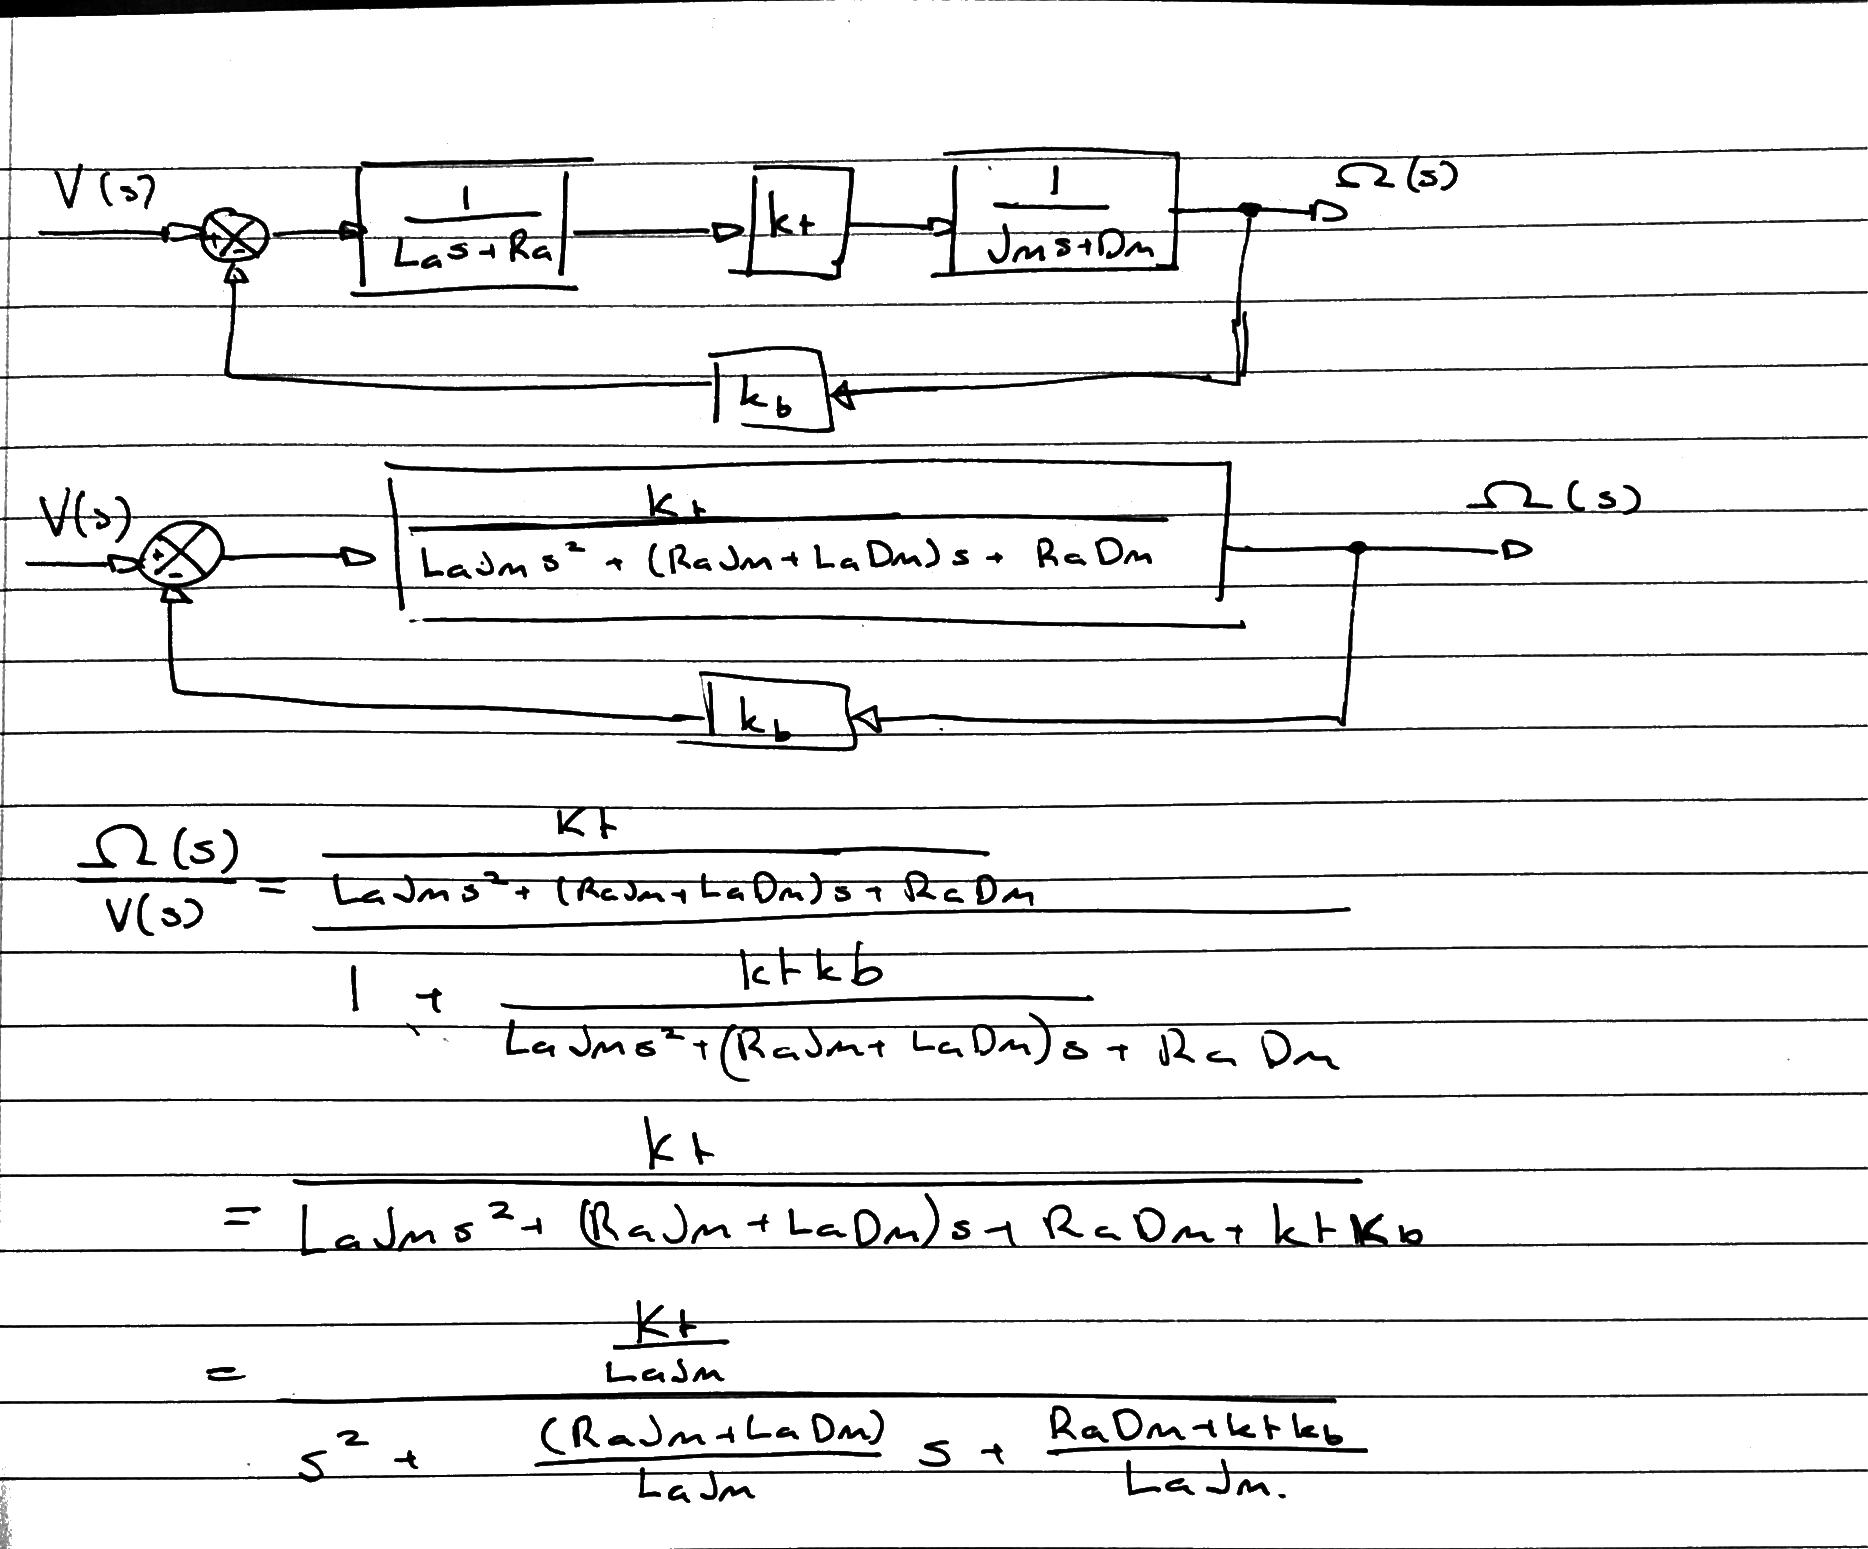
\includegraphics[width=\columnwidth]{lab2Derivation.jpg}
                \caption{Full derivation of \cref{fig:motorBlockDiagramValues} from block diagram to transfer function}
                \label{fig:motorDerivation}
            \end{figure}

        \section{Manual Derivation of A and B for an Unpowered Damped Pendulum}\label{app:AB}
            \begin{figure}[!h]
                \centering
                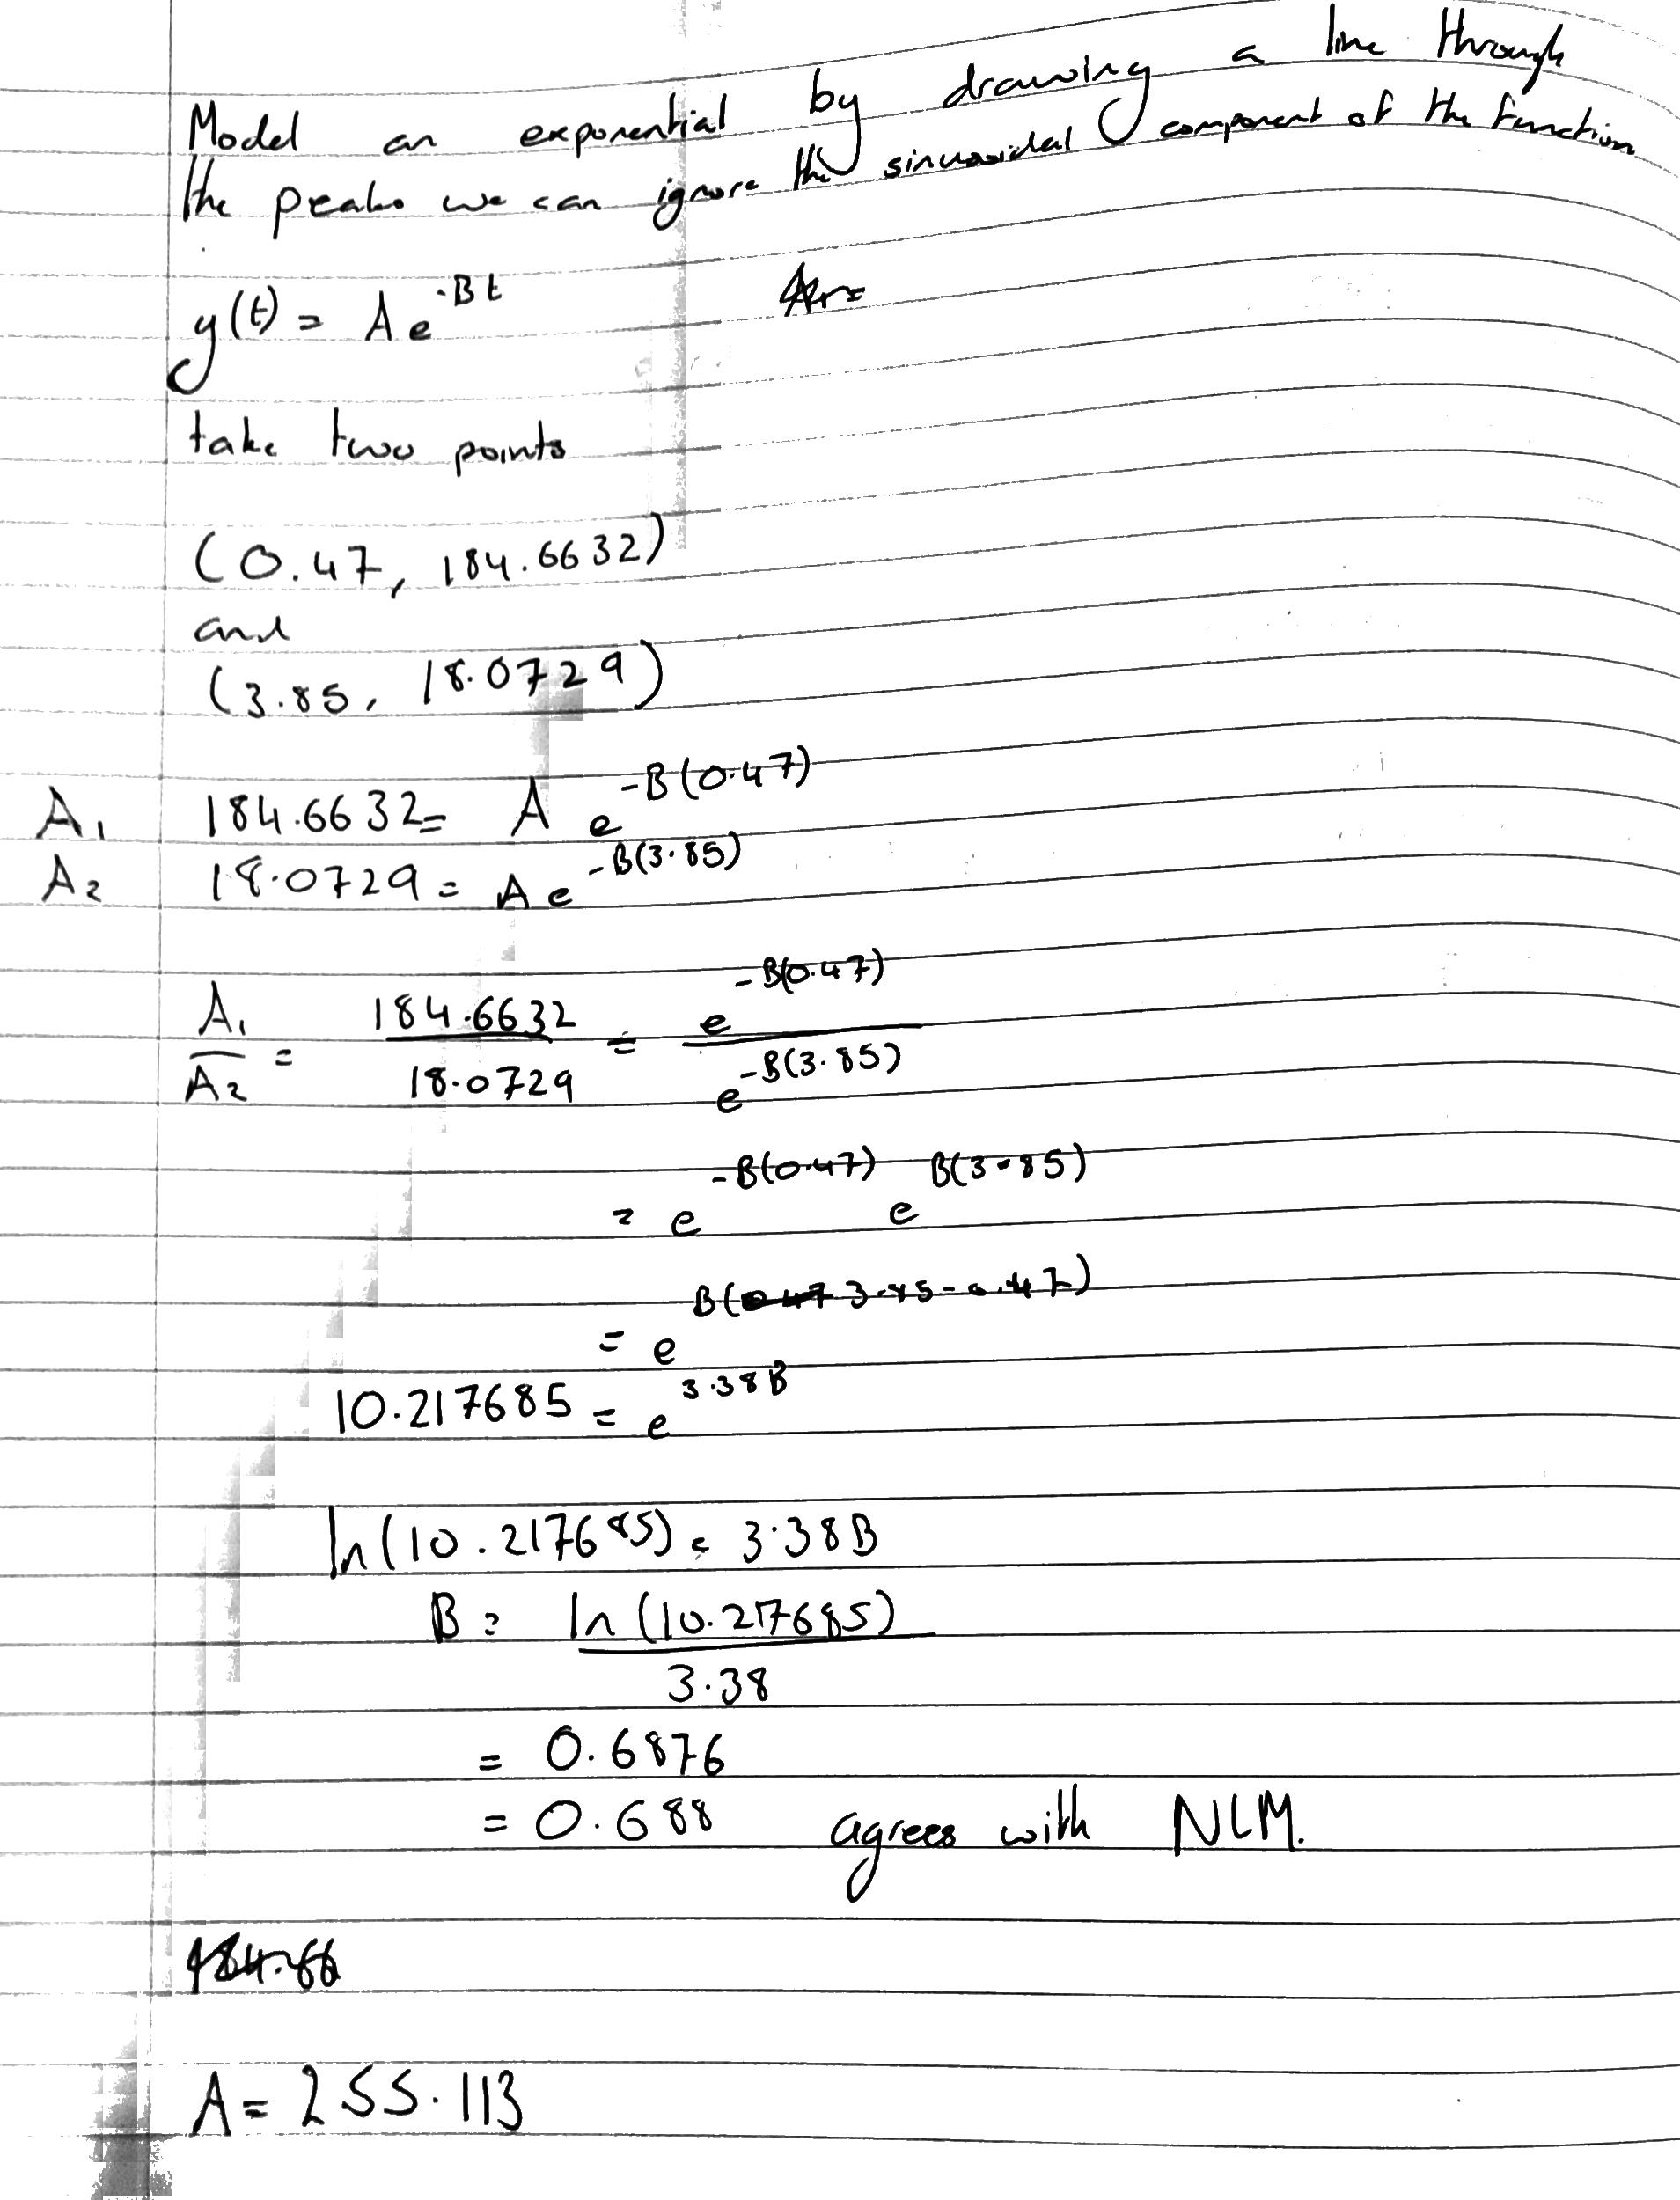
\includegraphics[width=0.9\columnwidth]{AB.jpg}
                \caption{Working for finding A and B using two peaks of a damped sinusoid}
                \label{fig:workingAB}
            \end{figure}
        \section{Manual Derivation of the final systems Transfer Function}\label{app:fullTF}
            \begin{figure}[!h]
                \centering
                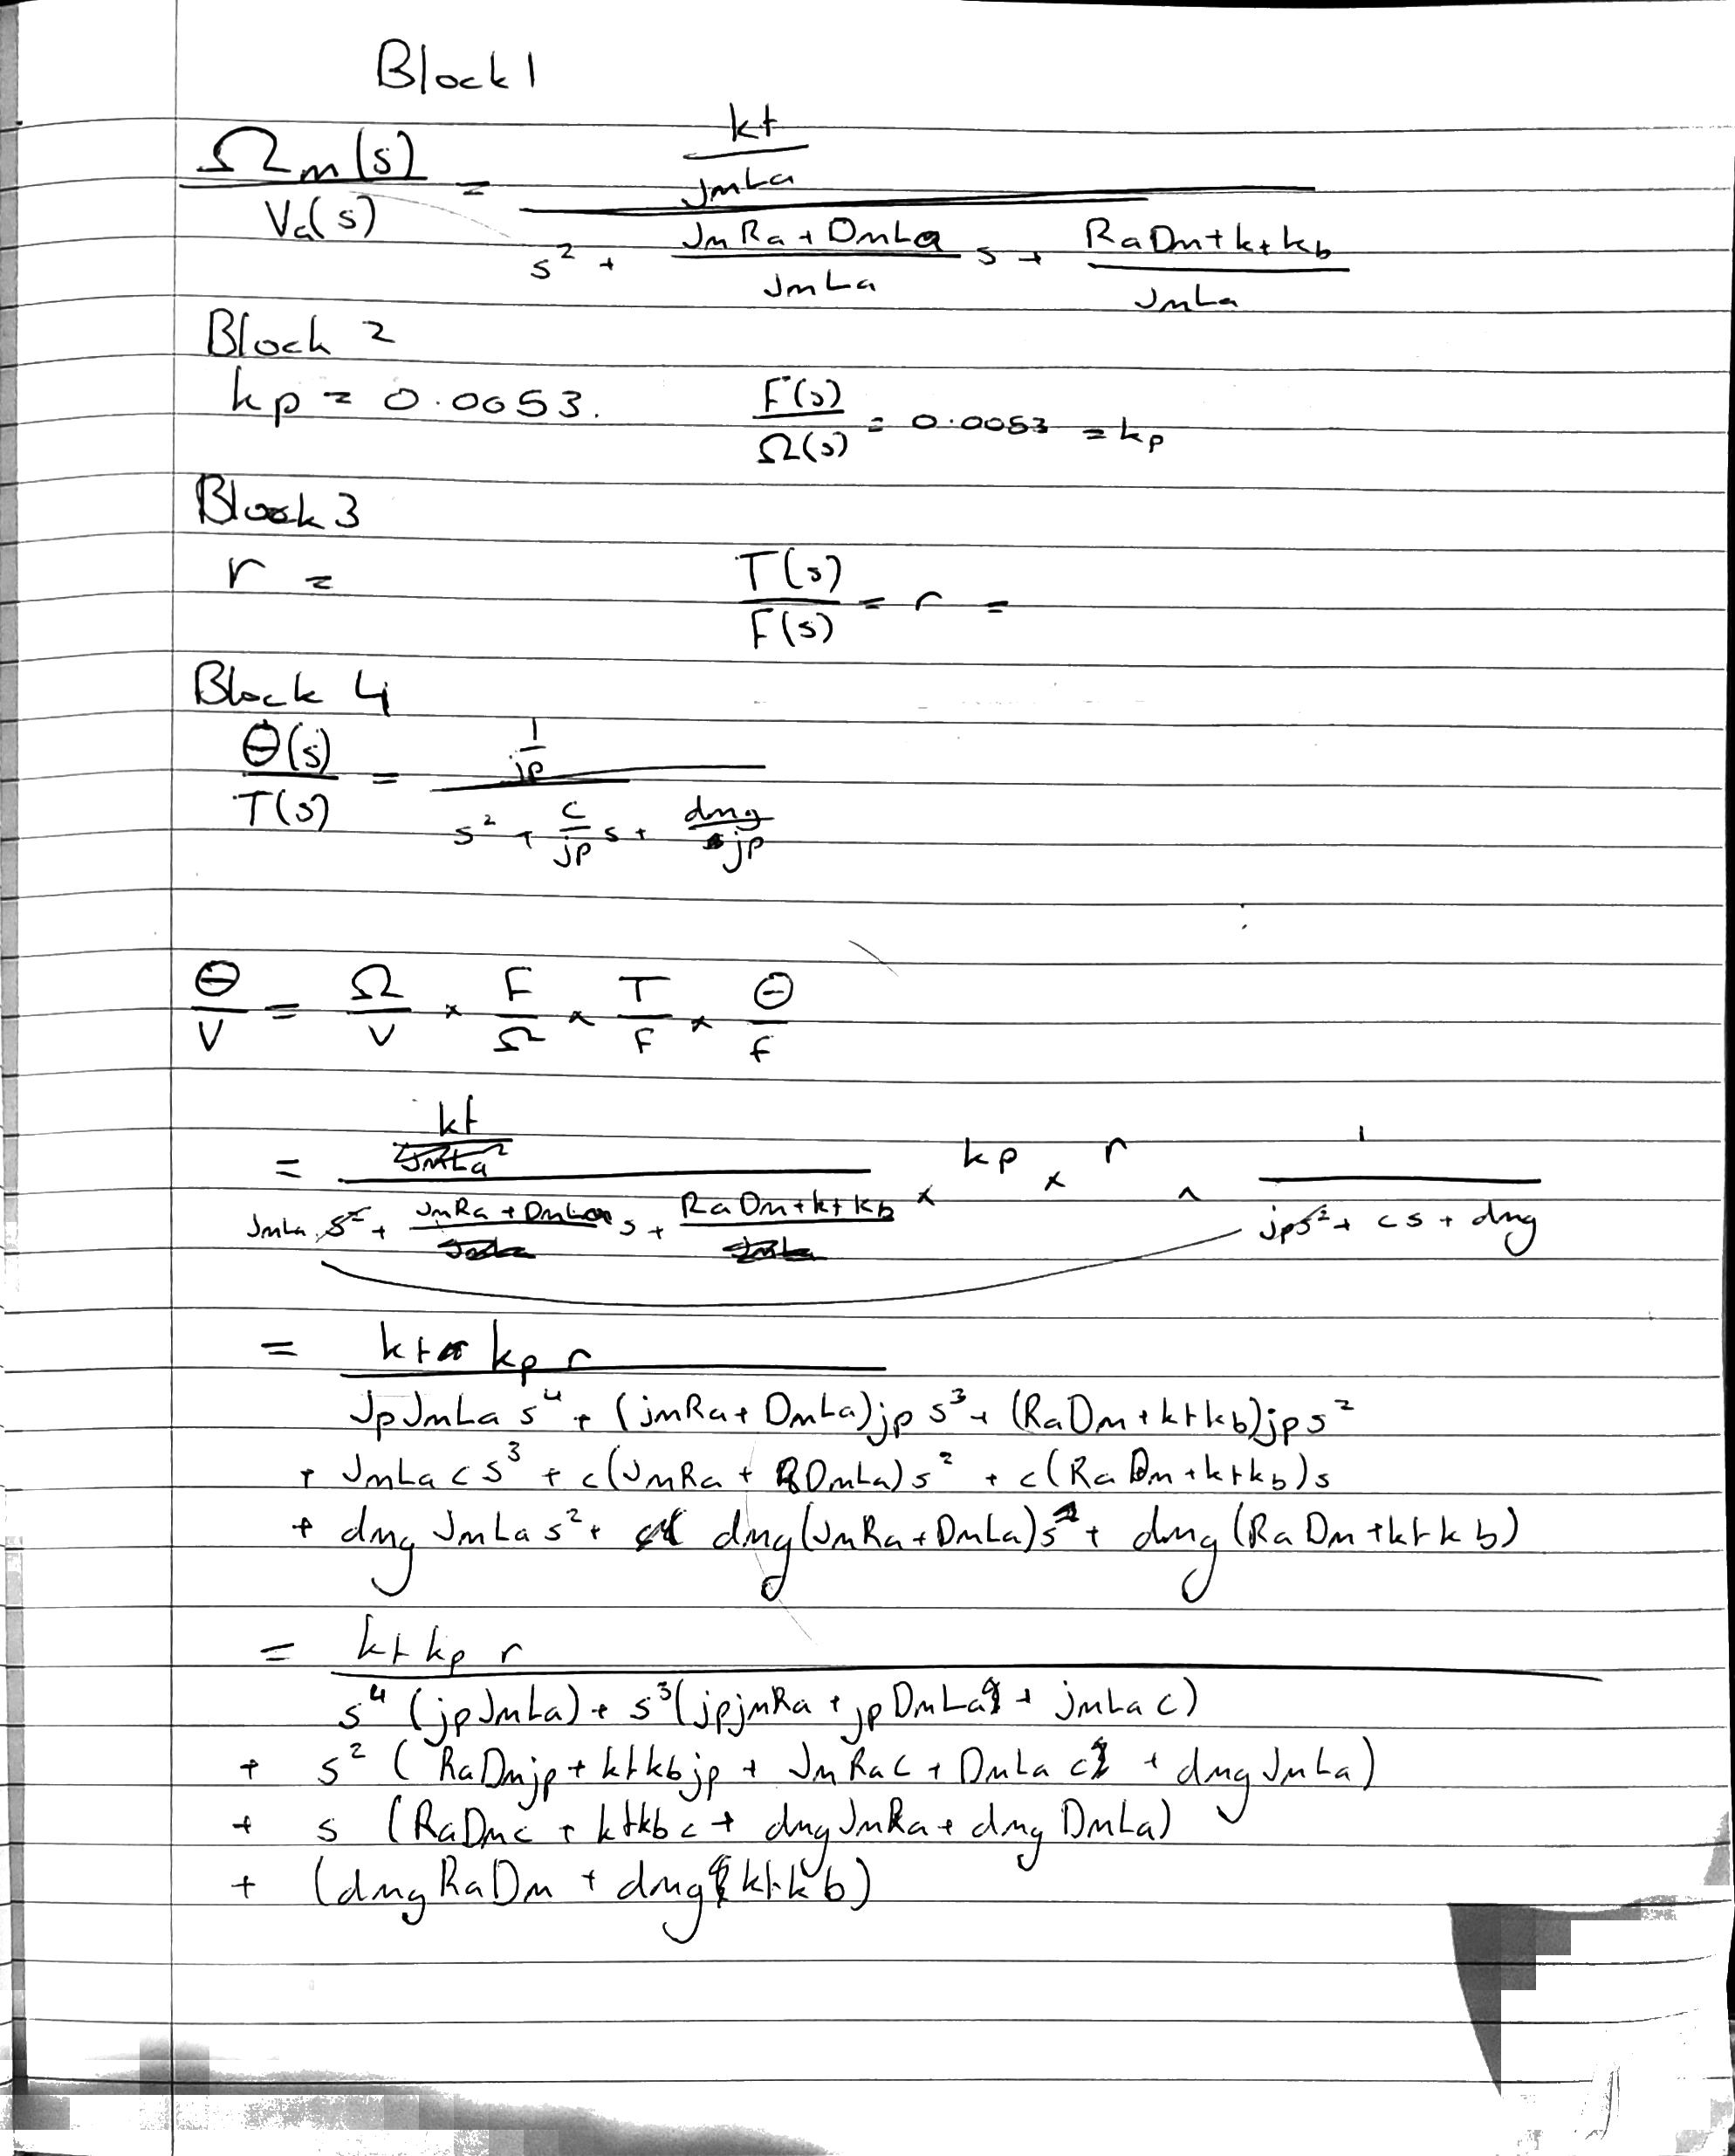
\includegraphics[width=\columnwidth]{fullTFDerivation.jpg}
                \caption{Working to find the full systems transfer function}
                \label{fig:workingTF}
            \end{figure}

\end{document}